\section{Ziel}
Das Ziel dieses Versuchs ist es die Strahlendosis und die
Strahlungsleistung in einem mit Röntgenstrahlung bestrahlten
Luftvolumen zu bestimmen.

\section{Theorie}
\label{sec:Theorie}

Die Dosimetrie ist die Lehre von den Verfahren zur Messung 
der von einem System aufgenommenen Dosis bzw. Dosisleistung.
Es wird die mit der ionisierenden Strahlung
verbundene Strahlenwirkung gemessen.


\subsection{Ionendosis J und Ionendosisrate j}
Mit der Ionisation des bestrahlten Materials geht zumeist
eine Absorption von Röntgenstrahlung einher. %gleiche Formulierung wie in der Anleitung
Die Ionendosis ist durch die in Luft erzeugte Ladung $dQ$
relativ zur Masse $dm_\text{L}$ der bestrahlten Luft definiert:
\begin{equation*}
    J = \frac{dQ}{dm_\text{L}}.
    \label{eqn:Ionendosis}
\end{equation*}

Die Ionendosisrate $\dot{J}$ entspricht dem zeitlichen Differential der Ionendosis $J$, also gilt 
\begin{equation}
    j = \dot{J} =\frac{dQ}{dt} \frac{1}{dm_\text{L}} =\frac{I}{dm_\text{L}} .
    \label{eqn:Ionendosis}
\end{equation}

\subsection{Energiedosis D und die mittlere Energiedosisrate d}
Die Energiedosis ist das Verhältnis von absorbierter
Energie $dE$ zu der Masse $dm$ des Absorbers.
Sie wird beschrieben durch
\begin{equation*}
    D = \frac{dE}{dm} = \frac{1}{\rho} * \frac{dE}{dV}.
    \label{eqn:Energiedosis}
\end{equation*}
Dabei ist $\rho$ die Dichte des Absorbers.
Die Energiedosisrate $\dot{D}$ ergibt sich im Mittel zu 
\begin{equation}
    d = \dot{D}_\text{m} = \frac{D}{t} =\frac{E}{m \cdot t} = n \cdot \Phi = \frac{j \cdot \Phi}{e}.
    \label{eqn:Energiedosisrate}
\end{equation}
Dabei ist $\Phi$ die Ionisationsenergie, $n$ die Anzahl der Ionen pro Kilogramm und pro Sekunde. 
Diese ergibt sich zu
\begin{equation*}
    n = \frac{j}{e},
    \label{eqn:Ionenanzahl}
\end{equation*}
wobei $e$ der Elementarladung entspricht. 

\subsection{Äquivalenzdosis H}
Die Wirkung ionisierender Strahlung auf biologische Materie
hängt bei gleicher Energiedosis von der Art der ionisierenden
Strahlung ab. Dieser Einfluss der Strahlungsenergie und -art
auf die biologische Wirkung wird durch den Qualitätsfaktor,
den Faktor der relativen biologischen Wirkung,
beschrieben.
Die Äquivalenzdosis $H$ kann durch diesen Qualitätsfaktor
berechnet werden:
\begin{equation*}
    H = Q * \frac{dE}{dm} = Q * D.
    \label{eqn:Aequivalenzdosis}
\end{equation*}

\subsection{Dosisleistung}
Die Dosisleistung ist jeweils die Dosis pro Zeiteinheit.
Kurven gleicher Dosisleistung sind sogenannte Isodosen.

\subsection{Bestrahlung eines Luftvolumens mit Röntgenstrahlung}
Wird ein Luftvolumen in einem Plattenkondensator
(siehe Abb. \ref{fig:Strahlgeometrie}) mit
Röntgenstrahlung bestrahlt und ionisiert, erzeugen die durch
den Röntgenstrahl erzeugten Ionen und Elektronen einen Strom.
Dieser Strom wächst mit steigender Kondensatorspannung 
$U_\text{K}$ an bis er den Sättigungsstrom $I_\text{S}$
erreicht. Mithilfe dieses Stroms können die dosimetrischen
Größen bestimmt werden.
\newline
Das ionisierte Luftvolumen kann folgendermaßen bestimmt werden:
\begin{equation*}
    V = \frac{1}{3} \pi (R^2 (x_0 + x_1 + x_2) - r^2 (x_0 + x_1)). 
\end{equation*}
Dabei sind die Radien
\begin{align*}
    R &= \frac{d \, x_2}{2 \, x_0} \\
    r &= \frac{d \, x_1}{2 \, x_0}. 
\end{align*}
Das Volumen ist also 
\begin{equation}
    V = \frac{1}{3} \pi \left(\frac{d^2 x_2^2}{4 x_0^2}(x_0 + x_1 + x_2) - \frac{d^2 x_1^2}{4 x_0^2}(x_0 + x_1)\right).
    \label{eqn:V}
\end{equation}

\begin{figure}
    \centering
    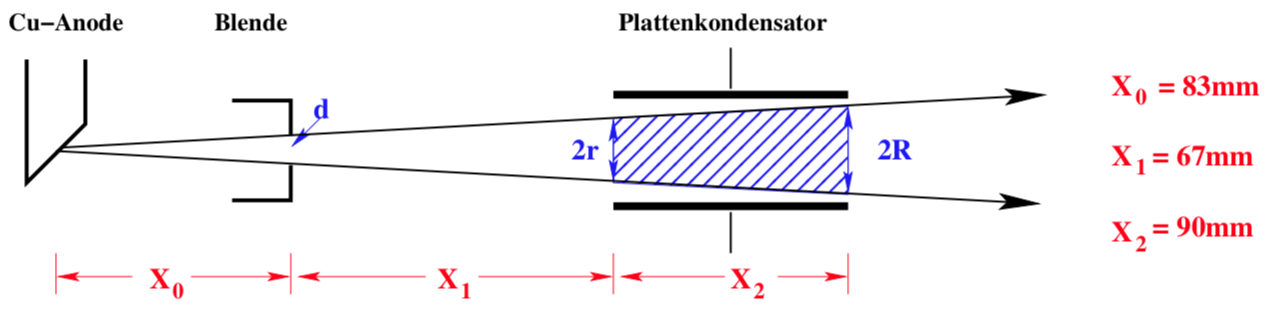
\includegraphics[width=12cm, height=4cm]{build/strahl.png}
    \caption{Skizze der Apparatur und des Strahlengangs. \cite{V607}}
    \label{fig:Strahlgeometrie}
\end{figure}
